\documentclass{standalone}
\usepackage{standalone}
\usepackage{siunitx}

\begin{document}
  \section{Architecture}
  In this diagram, the \textit{Can't Touch This} platform displayed globally.
  It shows three main objects:
  \begin{itemize}
    \tightlist{}
    \item The user
    \item The LeapMotion device
    \item The Can't Touch This platform
  \end{itemize}

  \begin{figure}[h]
    \centering
      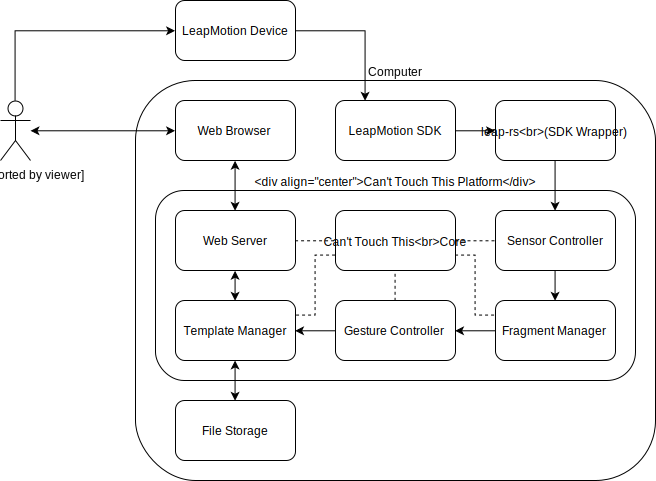
\includegraphics[width=\linewidth]{context-diagram}
    \caption{Context Diagram}
    \label{fig:context-diagram}
  \end{figure}

  The user attaches the LeapMotion device to the computer, installs the platform
  with it's required dependencies and moves it's hand above the sensor to
  conduct an experiment. The LeapMotion device shown at the top of figure~\ref{fig:context-diagram}
  above acts similar to a webcam, and captures visual data which is send to the
  computer the device is attached to. The LeapMotion SDK (daemon) running on
  this machine uses this visual data to detect hands a user is hovering above
  the sensor.

  \subsection{Library}
  In this section we describe what external components the application consists
  off to use the LeapMotion sensor.
  These are software parts required for the platform to work, but aren't
  part of the software application we developed itself.

  \subsubsection{LeapMotion SDK}
  This LeapMotion SDK consists of various components, as listed below:
  \begin{itemize}
    \tightlist{}
    \item Daemon: \textit{%
        A piece of software running on the host computer, to manage and talk
        to physical LeapMotion sensors connected to the computer.
      }
    \item Library: \textit{%
        The software library that can be used to talk to the daemon through
        your own software which supports various programming languages, to
        obtain sensor data. The daemon must of course be running in order for
        it to work.
      }
    \item Control panel: \textit{%
        A tool included to manage LeapMotion sensors, the state of the daemon
        and other things.
      }
    \item Visualizer: \textit{%
        An application showing a 3D perspective of the detected hands, useful
        for visual sensor feedback.
      }
  \end{itemize}
  Along with the named components above, documentation and some examples are
  included as well.

  \subsubsection{Rust \& Wrapper}
  We've decided to write our platform in the Rust programming language. There is
  no native LeapMotion library available for use with this language. Therefore
  we were required to use and develop a custom wrapper to translate parts of the
  provided library to something Rust supports, essentially being a Rust library.
  Our implementation is based on the open-source
  \href{https://github.com/panicbit/leap-rs}{leap-rs} project. This was the only
  Rust implementation of code that could talk to the LeapMotion library we could
  find.

  Because it was quite limited, we did
  \href{https://github.com/timvisee/leap-rs}{fork}
  the project to extend it with new functionality required for our project.
  For example, we added support for obtaining finger data being part of a hand.
  This allowed us to check what fingers were in view, what fingers were extended
  and so on.
  We did push our improvements to the upstream project, which were accepted and
  \href{https://github.com/panicbit/leap-rs/pulls?utf8=%E2%9C%93&q=is%3Apr+is%3Aclosed+author%3Atimvisee}{merged}!

  \begin{figure}[h]
    \centering
      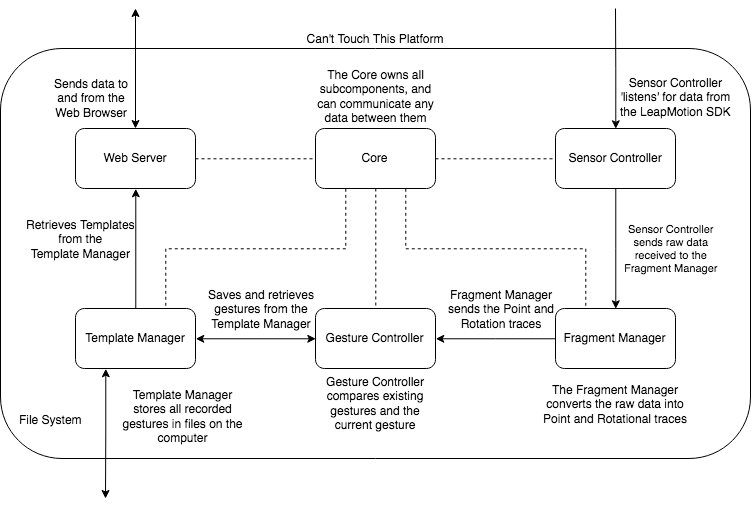
\includegraphics[width=\linewidth]{functional-diagram}
    \caption{Functional Diagram}
    \label{fig:pipeline-diagram}
  \end{figure}

  \subsection{Application}
  In this section we go over the different components inside the application.
  These components are better shown in the functional diagram,
  figure \ref{fig:pipeline-diagram}.

  \subsubsection{Sensor Controller}
  Our software, the respective platform, talks to the LeapMotion daemon being
  part of the LeapMotion SDK to obtain data from the sensor. This is done in the
  \verb_SensorController_ shown in the figure above. Note that the figure
  clearly visualizes that all communication with the LeapMotion SDK is done
  through the \verb_leap-rs_ wrapper. This is also the start of what we call
  \verb_the pipeline_ within our platform. This pipeline is a virtual concept
  for how data flows through our program, from raw sensor data to gesture
  detection.
  Figure~\ref{fig:pipeline-diagram} illustrates this in
  better detail.

  \subsubsection{Fragment Manager}
  The \verb_SensorController_ controls any connected sensors and attempts to
  collect sensor data, which it passes on to the \verb_FragmentManager_. This
  manager organizes and tracks sensor data. Raw incomming coordinate data is
  identified and grouped by hand and finger. Over a period of time the manager
  collects traces for detected fingers, which essentially define the path
  fingers have moved above the sensor until then. Along with collecting and
  organizing raw sensor data, the fragment manager processes the data into
  something we can easily use further down the \verb_pipeline_. In our case, we
  resample, scale, filter and map 3D point data into rotational point data.

  \paragraph{Resample}
  The LeapMotion sensor reports hand coordinate updates at varying rates, while
  the sensor is used. This causes collected 3D point data to have greatly
  varying distances between points, which makes further using the data quite a
  challenge. Therefore, the first step of processing the data is resampling 3D
  points with equal distance along the general curve the user had drawn above
  the sensor. The distance is small enough to represent the slightest curves and
  figures a user would intentionally perform, to ensure no important curve data
  is lost. Any exceptional disproportionate points are filtered from the stream
  of 3D points.

  \paragraph{}
  After resampling, the platform scales the drawn figure to a consistent size
  for easy comparison later on in the pipeline when attempting to detect
  gestures.

  \paragraph{Rotational trace}
  Lastly, we map the new list of 3D points into rotational data. To achieve
  this, we calculate the angle in 2D space between all 3D points. For each of
  these angles we determine the difference to define a new list of points having
  a relative rotation and a constant distance to the next point.
  This rotational data along with the point distance is sufficient for our logic,
  thus we throw away the 3D coordinate data and are left with a trace of
  rotational points.

  \paragraph{Example}
  To better illustrate the result data, here we'll go through two examples.
  Imagine drawing a perfectly straight line, this would map into a list of
  rotational points all having a relative rotation of 0\si{\degree} (degrees).
  The number of points would depend on how long the drawn line is, and what the
  constant distance is between the points when resampling.

  When drawing a perfect circle, the sensor data would map into a list of
  rotational points all having a relative rotation of about 15\si{\degree}. The
  smaller the radius of the circle, the larger the relative rotation would
  become. When drawing the circle the other way around, the relative rotation
  for each point would be negated.

  \paragraph{}
  You can probably imagine that this rotational trace data is good enough to
  define an abstract variant of a figure a user has drawn with his
  finger, as this data defines the distance and curve a finger has been moved.
  This is exactly what we're using and are doing comparisons with while
  attempting to detect gestures, comparing the general figure of a curve being
  performed by a user.

  \subsubsection{Gesture Controller}
  For each new data point being collected by the \verb_FragmentManager_, the
  then processed data is passed to the \verb_GestureController_. Here is where
  the gesture detection magic happens. This controller connects to the
  \verb_TemplateManager_ which holds a database of known gestures that a user
  has defined.

  The controller is constantly comparing incoming data against all
  defined templates until a match is found for the curve a user is currently
  performing. Simply said; this is done by walking through all rotational points
  for the current rotational trace and all rotational traces from all templates
  from the end (the newest point) to the beginning (the oldest point). If a
  template trace starts to differentiate too much from the current curve, that
  option is dropped. If walking through a template trace fully succeeds, a
  match is found.

  Some constants and thresholds are used to determine whether a
  step is allowed when walking through, these are configurable in the source
  code of our platform itself. This allows testing of various threshold
  configurations for determining what produces the most accurate results.
  When a match is found, the user is notified with the name of the template that
  was detected.

  \paragraph{}
  We choose this approach with a custom gesture recognition system, because we
  were unable to find a Rust library that did have support for gesture
  recognition. Also, outside the scope of Rust the detection libraries are
  severely limited. Some are limited to a few hard-coded gestures and don't
  support shape matching. Implementations for touchpads on laptops are
  proprietary.

  The LeapMotion SDK implements basic gesture recognition itself. This is
  however limited to a few static actions. Namely:
  \begin{itemize}
    \tightlist{}
    \item A circle gesture
    \item A swipe gesture
    \item A tap gesture
  \end{itemize}
  The SDK doesn't support adding more gestures. And, because the SDK is
  proprietary we were not able to extract the detection logic from this to
  implement ourselves.

  The Xbox Kinect had a few interesting gesture recognition libraries. One of
  these is \href{https://archive.codeplex.com/?p=kinectdtw}{KinectDTW}. This
  library is also limited to some very basic actions, and wasn't viable for our
  purpose.

  The
  \href{https://forums.leapmotion.com/t/openleapkit-updated-leap-motion-controller-toolkit-for-common-needs/289}{OpenLeapKit}
  project provided some awesome resources, but didn't really get into actual
  dynamic gesture recognition.

  Two forum posts discussing hand gesture detection suggested to use an machine
  learning approach, for which you train a detection model. This wasn't a viable
  option for us though, as such models need to be trained with a lot of data.
  Doing this physically isn't really possible, thus we'd have to build a
  simulator and generate a lot of sample data to train. Building this would be a
  project on it's own.

  \paragraph{}
  In the end we came across
  \href{http://www.creativedistraction.com/demos/gesture-recognition-kinect-with-hidden-markov-models-hmms/}{HMM}
  (Hidden Markov Models), and the term
  \href{http://delivery.acm.org/10.1145/3140000/3134139/p12-balcazar.pdf}{Circular
  Measurements}, the two seemingly go-to methods for doing gesture recognition
  in our context.

  After researching both we did decide to go with the latter.
  Not just because it seemed to be simpler to implement. But also because it is
  must more dynamic because it only compares and tries to match two gestures,
  and didn't require us to specify (and/or train) detection models.
  Recording a new gesture with the \emph{Circular Measurement} method is as
  simple as converting the sensor data to data we normally use within the
  platform, and collecting it to a file to compare new gestures against later.

  We thought implementing a system for this was an awesome challenge to use for
  gesture recognition.

  \subsubsection{Web interface}
  The platform provides a web interface for control. First of all, this
  interface provides a real-time visualiser for the processed sensor data. To
  achieve this, the web backend in our platform talks to various components in
  the \verb_pipeline_ of the application. The visualizer clearly shows the
  current curve a user has drawn, along with the resample points. This visual
  feedback should improve the quality of gestures users can perform as users
  can adapt to what they're seeing is being detected.

  Templates are also managed through this interface as stored in the
  \verb_TemplateManager_, for recording new templates and removing existing
  ones. When recording a new template, the visualizer shows the current state
  of the drawn figure until the user stops the recording. Recorded gestures can
  then be trimmed through the interface to cut off unwanted parts.

  \paragraph{}
  File storage is used to store user defined templates on the host machine, to
  properly remember templates across platform restarts. File storage has been
  chosen in contrast to a fully featured database, as it makes the platform much
  easier to set up.

  \paragraph{}
  When looking at the live visualizer for the first time, you might see that the
  visualized figure is drawn in a different orientation than your performed
  gesture above the sensor. This is a side effect of the data we're using. The
  shown gestures are based on data after processing in the
  \verb_FragmentManager_. As noted, this only outputs relative rotation data
  along with a constant distance. Because the rotation is relative the
  visualizer has no concept of in what real-world orientation the gesture is
  performed. The visualizer always starts drawing the processed trace into the
  same direction (form the center of the visualizer, toward the left of the
  screen). This does not affect the actual detection at all. And in our opinion
  it isn't important enough to include the rotation relative to the world just
  to better visualize the performed gesture.

  \clearpage
\end{document}
